% % % % % % % % % % % % % % % % % % % %

\part{Connecting Coding and \newline
Compressed Sensing via \newline
Approximate Message Passing}
\frame{\partpage}

% % % % % % % % % % % % % % % % % % % %

\begin{frame}
\frametitle{Coded Compressive Sensing -- Divide and Conquer}
% % % % %
\begin{center}
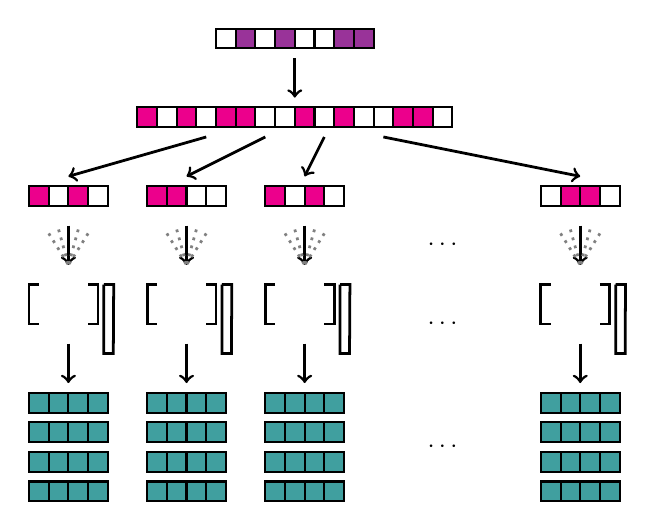
\begin{tikzpicture}
[font=\small, draw=black, line width=0.75pt,
sub0/.style={rectangle, draw, inner sep=0pt, minimum width=10mm, minimum height=2.5mm},
parity/.style={rectangle, draw, fill=teal!75, inner sep=0pt, minimum size=2.5mm},
bit0/.style={rectangle, draw, inner sep=0pt, minimum size=2.5mm},
bit1/.style={rectangle, draw, fill=violet!80, inner sep=0pt, minimum size=2.5mm},ebit0/.style={rectangle, draw, inner sep=0pt, minimum size=2.5mm},
ebit1/.style={rectangle, draw, fill=magenta, inner sep=0pt, minimum size=2.5mm}
]

\node[bit0] (info0) at (1.00,8.125) {};
\node[bit1] (info1) at (1.25,8.125) {};
\node[bit0] (info2) at (1.50,8.125) {};
\node[bit1] (info3) at (1.75,8.125) {};
\node[bit0] (info4) at (2.00,8.125) {};
\node[bit0] (info5) at (2.25,8.125) {};
\node[bit1] (info6) at (2.50,8.125) {};
\node[bit1] (info7) at (2.75,8.125) {};

\draw[->, line width=1pt]  (1.875,7.875) -- (1.875,7.375);

\node[ebit1] (bit0) at (0.00,7.125) {};
\node[ebit0] (bit1) at (0.25,7.125) {};
\node[ebit1] (bit2) at (0.50,7.125) {};
\node[ebit0] (bit3) at (0.75,7.125) {};
\node[ebit1] (bit4) at (1.00,7.125) {};
\node[ebit1] (bit5) at (1.25,7.125) {};
\node[ebit0] (bit6) at (1.50,7.125) {};
\node[ebit0] (bit7) at (1.75,7.125) {};
\node[ebit1] (bit8) at (2.00,7.125) {};
\node[ebit0] (bit9) at (2.25,7.125) {};
\node[ebit1] (bit10) at (2.50,7.125) {};
\node[ebit0] (bit11) at (2.75,7.125) {};
\node[ebit0] (bit12) at (3.00,7.125) {};
\node[ebit1] (bit13) at (3.25,7.125) {};
\node[ebit1] (bit14) at (3.50,7.125) {};
\node[ebit0] (bit15) at (3.75,7.125) {};

\draw[->, line width=1pt]  (0.75,6.875) -- (-1.00,6.375);
\draw[->, line width=1pt]  (1.50,6.875) -- (0.50,6.375);
\draw[->, line width=1pt]  (2.25,6.875) -- (2.00,6.375);
\draw[->, line width=1pt]  (3.00,6.875) -- (5.50,6.375);

\node[ebit1] (s00) at (-1.375,6.125) {};
\node[ebit0] (s01) at (-1.125,6.125) {};
\node[ebit1] (s02) at (-0.875,6.125) {};
\node[ebit0] (s02) at (-0.625,6.125) {};

\node[ebit1] (s03) at (0.125,6.125) {};
\node[ebit1] (s04) at (0.375,6.125) {};
\node[ebit0] (s05) at (0.625,6.125) {};
\node[ebit0] (s05) at (0.875,6.125) {};

\node[ebit1] (s06) at (1.625,6.125) {};
\node[ebit0] (s07) at (1.875,6.125) {};
\node[ebit1] (s08) at (2.125,6.125) {};
\node[ebit0] (s08) at (2.375,6.125) {};

\node[ebit0] (s09) at (5.125,6.125) {};
\node[ebit1] (s10) at (5.375,6.125) {};
\node[ebit1] (s11) at (5.625,6.125) {};
\node[ebit0] (s11) at (5.875,6.125) {};

\foreach \v in {-1.00,0.50,2.00,5.50} {
  \draw[->, line width=1pt]  (\v,4.25) -- (\v,3.75);
  \draw[->, line width=1pt]  (\v,5.75) -- (\v,5.25);
  \draw[dotted, line width=1pt, draw=gray]  (\v-0.25,5.65) -- (\v,5.25);
  \draw[dotted, line width=1pt, draw=gray]  (\v-0.125,5.7) -- (\v,5.25);
  \draw[dotted, line width=1pt, draw=gray]  (\v+0.125,5.7) -- (\v,5.25);
  \draw[dotted, line width=1pt, draw=gray]  (\v+0.25,5.65) -- (\v,5.25);
}

\node (dots1) at (3.75,5.5) {$\cdots$};

\foreach \v in {-1.00,0.50,2.00,5.50} {
  \draw[line width=1pt] (\v-0.375,5) -- (\v-0.5,5) -- (\v-0.5,4.5) -- (\v-0.375,4.5);
  \draw[line width=1pt] (\v+0.25,5) -- (\v+0.375,5) -- (\v+0.375,4.5) -- (\v+0.25,4.5);
  \draw[line width=1pt] (\v+0.45,5) -- (\v+0.45,4.125) -- (\v+0.57,4.125) -- (\v+0.575,5) -- (\v+0.45,5);
}

\node (dots2) at (3.75,4.5) {$\cdots$};
\node (dots3) at (3.75,2.9375) {$\cdots$};

\foreach \c in {3.50, 3.125, 2.75, 2.375} {
  \node[parity] (subcs00c\c) at (-1.375,\c) {};
  \node[parity] (subcs01c\c) at (-1.125,\c) {};
  \node[parity] (subcs02c\c) at (-0.875,\c) {};
  \node[parity] (subcs02c\c) at (-0.625,\c) {};

  \node[parity] (subcs03c\c) at (0.125,\c) {};
  \node[parity] (subcs04c\c) at (0.375,\c) {};
  \node[parity] (subcs05c\c) at (0.625,\c) {};
  \node[parity] (subcs05c\c) at (0.875,\c) {};

  \node[parity] (subcs06c\c) at (1.625,\c) {};
  \node[parity] (subcs07c\c) at (1.875,\c) {};
  \node[parity] (subcs08c\c) at (2.125,\c) {};
  \node[parity] (subcs08c\c) at (2.375,\c) {};

  \node[parity] (subcs09c\c) at (5.125,\c) {};
  \node[parity] (subcs10c\c) at (5.375,\c) {};
  \node[parity] (subcs11c\c) at (5.625,\c) {};
  \node[parity] (subcs11c\c) at (5.875,\c) {};
}

\end{tikzpicture}

\end{center}
\begin{itemize}
\item Data fragmentation and indexing
\item Outer encoding for disambiguation
\end{itemize}
\end{frame}

% % % % % % % % % % % % % % % % % % % %

\begin{frame}
\frametitle{CCS -- Approximate Message Passing}
\begin{center}
\begin{tikzpicture}
  \node[scope fading=south] (image) at (0,0) {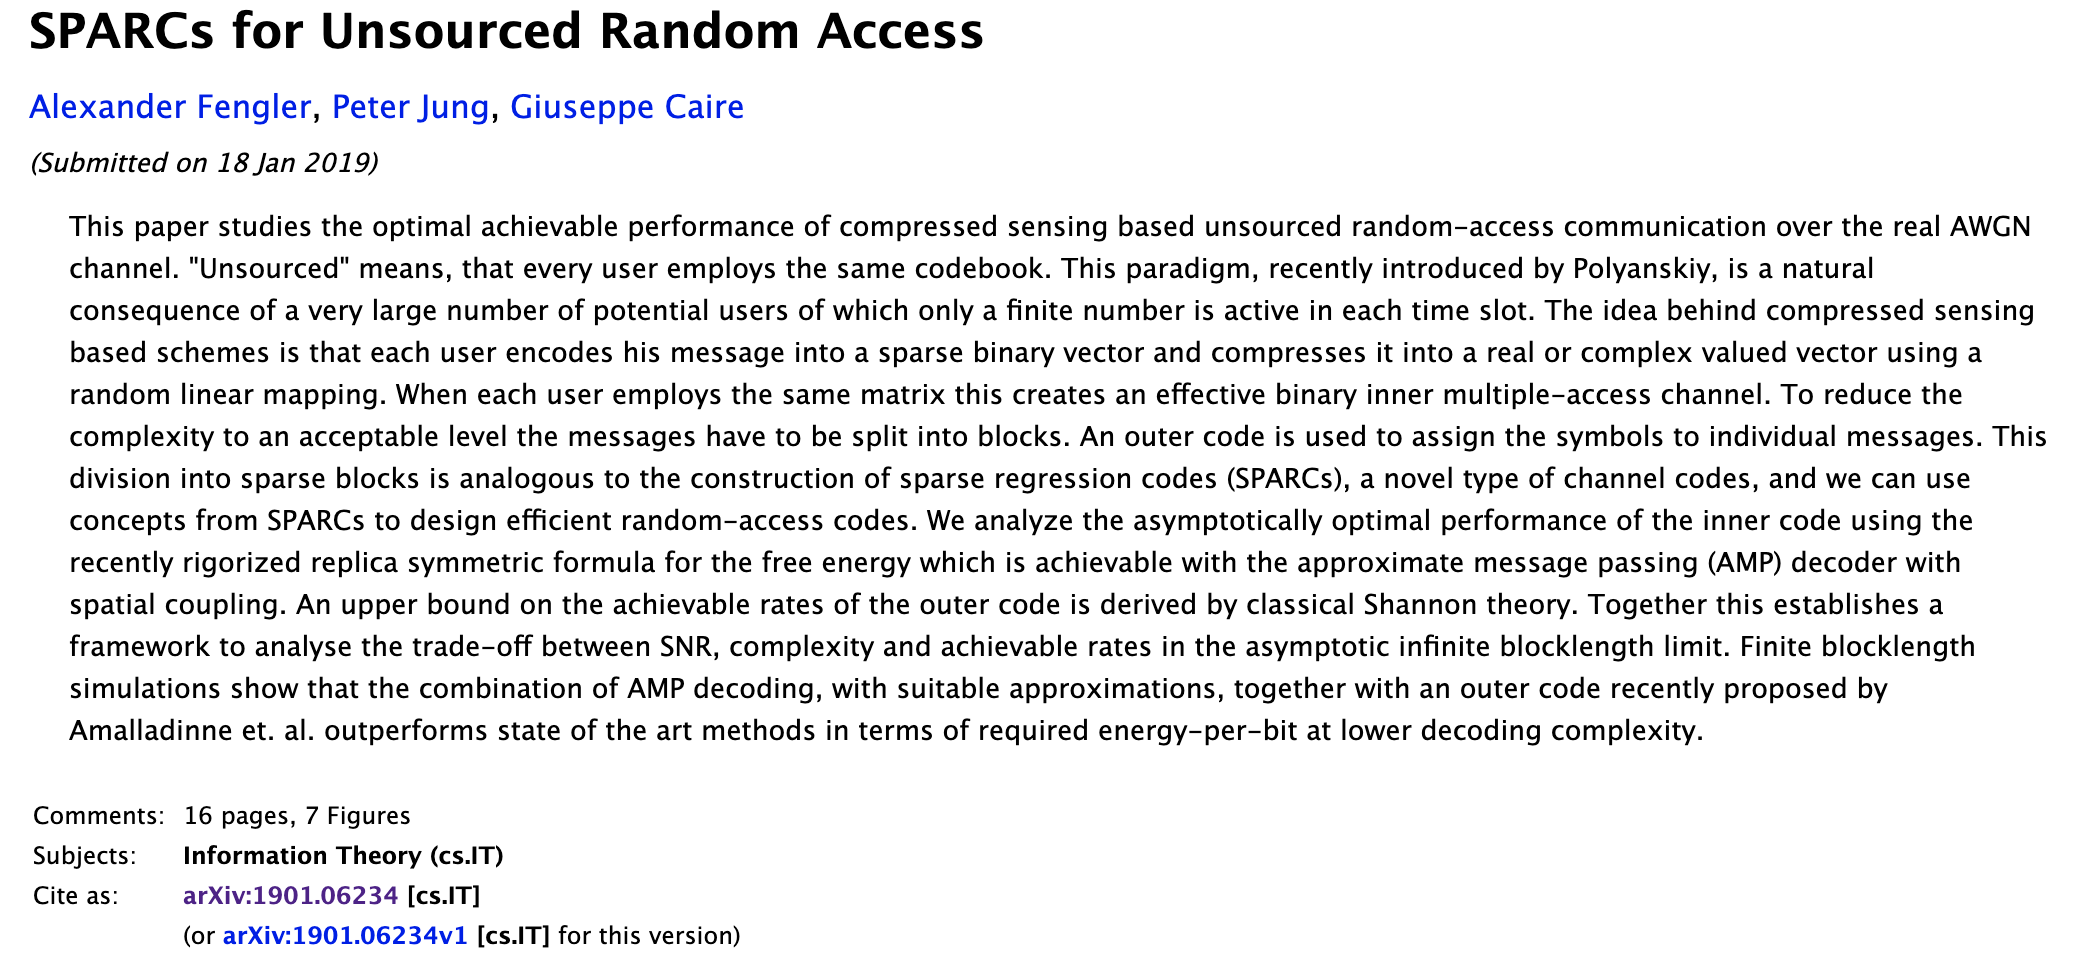
\includegraphics[width=4in]{Figures-AMP/SparcsUMAC.png}};
\end{tikzpicture}
\end{center}
  \begin{itemize}
  \item Connection between CCS indexing and sparse regression codes
  \item Circumvent slotting under CCS and dispersion effects
  \item Introduce denoiser tailored to CCS
  \end{itemize}
\end{frame}

% % % % % % % % % % % % % % % % % % % %

\begin{frame}
\frametitle{CCS Revisited}
\begin{center}
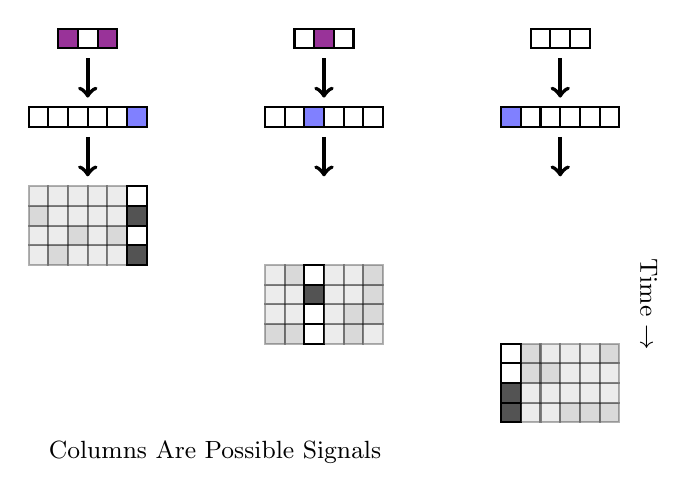
\begin{tikzpicture}
[font=\small, draw=black, line width=0.75pt,
bit0/.style={rectangle, draw, inner sep=0pt, minimum size=2.5mm},
bit1/.style={rectangle, draw, fill=violet!80, inner sep=0pt, minimum size=2.5mm},
entry0/.style={rectangle, draw, opacity=0.3, fill=lightgray, inner sep=0pt, minimum size=2.5mm},
entry1/.style={rectangle, draw, opacity=0.3, fill=gray, inner sep=0pt, minimum size=2.5mm},
entry00/.style={rectangle, draw, fill=white, inner sep=0pt, minimum size=2.5mm},
entry11/.style={rectangle, draw, fill=darkgray!90, inner sep=0pt, minimum size=2.5mm},
symbol0/.style={rectangle, draw, fill=white, inner sep=0pt, minimum size=2.5mm},
symbol1/.style={rectangle, draw, fill=blue!50, inner sep=0pt, minimum size=2.5mm}]

\node[entry11] (m2400) at (6.00,0) {};
\node[entry0] (m2500) at (6.25,0) {};
\node[entry0] (m2600) at (6.50,0) {};
\node[entry1] (m2700) at (6.75,0) {};
\node[entry1] (m2800) at (7.00,0) {};
\node[entry1] (m2900) at (7.25,0) {};

\node[entry11] (m2401) at (6.00,0.25) {};
\node[entry0] (m2501) at (6.25,0.25) {};
\node[entry0] (m2601) at (6.50,0.25) {};
\node[entry0] (m2701) at (6.75,0.25) {};
\node[entry0] (m2801) at (7.00,0.25) {};
\node[entry0] (m2901) at (7.25,0.25) {};

\node[entry00] (m2402) at (6.00,0.50) {};
\node[entry1] (m2502) at (6.25,0.50) {};
\node[entry1] (m2602) at (6.50,0.50) {};
\node[entry0] (m2702) at (6.75,0.50) {};
\node[entry0] (m2802) at (7.00,0.50) {};
\node[entry0] (m2902) at (7.25,0.50) {};

\node[entry00] (m2403) at (6.00,0.75) {};
\node[entry1] (m2503) at (6.25,0.75) {};
\node[entry0] (m2603) at (6.50,0.75) {};
\node[entry0] (m2703) at (6.75,0.75) {};
\node[entry0] (m2803) at (7.00,0.75) {};
\node[entry1] (m2903) at (7.25,0.75) {};

\node[entry1] (m1204) at (3.00,1.00) {};
\node[entry1] (m1304) at (3.25,1.00) {};
\node[entry00] (m1404) at (3.50,1.00) {};
\node[entry0] (m1504) at (3.75,1.00) {};
\node[entry1] (m1604) at (4.00,1.00) {};
\node[entry0] (m1704) at (4.25,1.00) {};

\node[entry0] (m1205) at (3.00,1.25) {};
\node[entry0] (m1305) at (3.25,1.25) {};
\node[entry00] (m1405) at (3.50,1.25) {};
\node[entry0] (m1505) at (3.75,1.25) {};
\node[entry1] (m1605) at (4.00,1.25) {};
\node[entry1] (m1705) at (4.25,1.25) {};

\node[entry0] (m1206) at (3.00,1.50) {};
\node[entry0] (m1306) at (3.25,1.50) {};
\node[entry11] (m1406) at (3.50,1.50) {};
\node[entry0] (m1506) at (3.75,1.50) {};
\node[entry0] (m1606) at (4.00,1.50) {};
\node[entry1] (m1706) at (4.25,1.50) {};

\node[entry0] (m1207) at (3.00,1.75) {};
\node[entry1] (m1307) at (3.25,1.75) {};
\node[entry00] (m1407) at (3.50,1.75) {};
\node[entry0] (m1507) at (3.75,1.75) {};
\node[entry0] (m1607) at (4.00,1.75) {};
\node[entry1] (m1707) at (4.25,1.75) {};

\node[entry0] (m0008) at (0.00,2.00) {};
\node[entry1] (m0108) at (0.25,2.00) {};
\node[entry0] (m0208) at (0.50,2.00) {};
\node[entry0] (m0308) at (0.75,2.00) {};
\node[entry0] (m0408) at (1.00,2.00) {};
\node[entry11] (m0508) at (1.25,2.00) {};

\node[entry0] (m0009) at (0.00,2.25) {};
\node[entry0] (m0109) at (0.25,2.25) {};
\node[entry1] (m0209) at (0.50,2.25) {};
\node[entry0] (m0309) at (0.75,2.25) {};
\node[entry1] (m0409) at (1.00,2.25) {};
\node[entry00] (m0509) at (1.25,2.25) {};

\node[entry1] (m0010) at (0.00,2.50) {};
\node[entry0] (m0110) at (0.25,2.50) {};
\node[entry0] (m0210) at (0.50,2.50) {};
\node[entry0] (m0310) at (0.75,2.50) {};
\node[entry0] (m0410) at (1.00,2.50) {};
\node[entry11] (m0510) at (1.25,2.50) {};

\node[entry0] (m0011) at (0.00,2.75) {};
\node[entry0] (m0111) at (0.25,2.75) {};
\node[entry0] (m0211) at (0.50,2.75) {};
\node[entry0] (m0311) at (0.75,2.75) {};
\node[entry0] (m0411) at (1.00,2.75) {};
\node[entry00] (m0511) at (1.25,2.75) {};

\draw[->, line width=1.5pt]  (0.625,3.50) -- (0.625,3.00);
\draw[->, line width=1.5pt]  (3.625,3.50) -- (3.625,3.00);
\draw[->, line width=1.5pt]  (6.625,3.50) -- (6.625,3.00);

\node[symbol0] (s00) at (0.00,3.75) {};
\node[symbol0] (s01) at (0.25,3.75) {};
\node[symbol0] (s02) at (0.50,3.75) {};
\node[symbol0] (s03) at (0.75,3.75) {};
\node[symbol0] (s04) at (1.00,3.75) {};
\node[symbol1] (s05) at (1.25,3.75) {};

\node[symbol0] (s12) at (3.00,3.75) {};
\node[symbol0] (s13) at (3.25,3.75) {};
\node[symbol1] (s14) at (3.50,3.75) {};
\node[symbol0] (s15) at (3.75,3.75) {};
\node[symbol0] (s16) at (4.00,3.75) {};
\node[symbol0] (s17) at (4.25,3.75) {};

\node[symbol1] (s24) at (6.00,3.75) {};
\node[symbol0] (s25) at (6.25,3.75) {};
\node[symbol0] (s26) at (6.50,3.75) {};
\node[symbol0] (s27) at (6.75,3.75) {};
\node[symbol0] (s28) at (7.00,3.75) {};
\node[symbol0] (s29) at (7.25,3.75) {};

\draw[->, line width=1.5pt]  (0.625,4.50) -- (0.625,4.00);
\draw[->, line width=1.5pt]  (3.625,4.50) -- (3.625,4.00);
\draw[->, line width=1.5pt]  (6.625,4.50) -- (6.625,4.00);

\node[bit1] (info0) at (0.375,4.75) {};
\node[bit0] (info1) at (0.625,4.75) {};
\node[bit1] (info2) at (0.875,4.75) {};
\node[bit0] (info3) at (3.375,4.75) {};
\node[bit1] (info4) at (3.625,4.75) {};
\node[bit0] (info5) at (3.875,4.75) {};
\node[bit0] (info6) at (6.375,4.75) {};
\node[bit0] (info7) at (6.625,4.75) {};
\node[bit0] (info8) at (6.875,4.75) {};


\node [anchor = west] (signals) at (0.00,-0.50) {Columns Are Possible Signals};
\node[rotate=-90] (time) at (7.75,1.375) {Time $\rightarrow$};
\end{tikzpicture}

\end{center}
\begin{itemize}
\item Bit sequence split into $L$ fragments
\item Each bit $+$ parity block converted to index in $[ 0, 2^{m/L}-1 ]$
\item Stack sub-codewords into $(n/L) \times 2^{m/L}$ sensing matrices
\end{itemize}
\end{frame}

% % % % % % % % % % % % % % % % % % % %

\begin{frame}
\frametitle{Coded Compressed Sensing -- Unified View}
% % % % %
\begin{center}
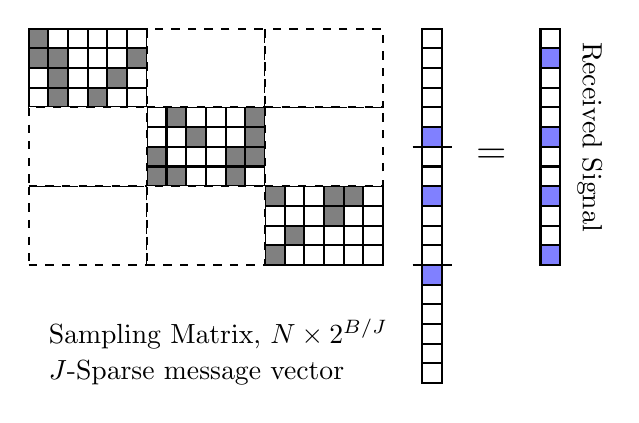
\begin{tikzpicture}
[draw=black, line width=0.75pt,
block/.style={rectangle, draw, fill=white, inner sep=0pt, minimum width=15mm,minimum height=10mm},
entry1/.style={rectangle, draw, fill=gray, inner sep=0pt, minimum size=2.5mm},
entry0/.style={rectangle, draw, fill=white, inner sep=0pt, minimum size=2.5mm},
symbol0/.style={rectangle, draw, fill=white, inner sep=0pt, minimum size=2.5mm},
symbol1/.style={rectangle, draw, fill=blue!50, inner sep=0pt, minimum size=2.5mm}]

\node[entry1] (m1800) at (4.50,0) {};
\node[entry0] (m1900) at (4.75,0) {};
\node[entry0] (m2000) at (5.00,0) {};
\node[entry0] (m2100) at (5.25,0) {};
\node[entry0] (m2200) at (5.50,0) {};
\node[entry0] (m2300) at (5.75,0) {};

\node[entry0] (m1801) at (4.50,0.25) {};
\node[entry1] (m1901) at (4.75,0.25) {};
\node[entry0] (m2001) at (5.00,0.25) {};
\node[entry0] (m2101) at (5.25,0.25) {};
\node[entry0] (m2201) at (5.50,0.25) {};
\node[entry0] (m2301) at (5.75,0.25) {};

\node[entry0] (m1802) at (4.50,0.50) {};
\node[entry0] (m1902) at (4.75,0.50) {};
\node[entry0] (m2002) at (5.00,0.50) {};
\node[entry1] (m2102) at (5.25,0.50) {};
\node[entry0] (m2202) at (5.50,0.50) {};
\node[entry0] (m2302) at (5.75,0.50) {};

\node[entry1] (m1803) at (4.50,0.75) {};
\node[entry0] (m1903) at (4.75,0.75) {};
\node[entry0] (m2003) at (5.00,0.75) {};
\node[entry1] (m2103) at (5.25,0.75) {};
\node[entry1] (m2203) at (5.50,0.75) {};
\node[entry0] (m2303) at (5.75,0.75) {};

\node[entry1] (m1204) at (3.00,1.00) {};
\node[entry1] (m1304) at (3.25,1.00) {};
\node[entry0] (m1404) at (3.50,1.00) {};
\node[entry0] (m1504) at (3.75,1.00) {};
\node[entry1] (m1604) at (4.00,1.00) {};
\node[entry0] (m1704) at (4.25,1.00) {};

\node[entry1] (m1205) at (3.00,1.25) {};
\node[entry0] (m1305) at (3.25,1.25) {};
\node[entry0] (m1405) at (3.50,1.25) {};
\node[entry0] (m1505) at (3.75,1.25) {};
\node[entry1] (m1605) at (4.00,1.25) {};
\node[entry1] (m1705) at (4.25,1.25) {};

\node[entry0] (m1206) at (3.00,1.50) {};
\node[entry0] (m1306) at (3.25,1.50) {};
\node[entry1] (m1406) at (3.50,1.50) {};
\node[entry0] (m1506) at (3.75,1.50) {};
\node[entry0] (m1606) at (4.00,1.50) {};
\node[entry1] (m1706) at (4.25,1.50) {};

\node[entry0] (m1207) at (3.00,1.75) {};
\node[entry1] (m1307) at (3.25,1.75) {};
\node[entry0] (m1407) at (3.50,1.75) {};
\node[entry0] (m1507) at (3.75,1.75) {};
\node[entry0] (m1607) at (4.00,1.75) {};
\node[entry1] (m1707) at (4.25,1.75) {};

\node[entry0] (m0608) at (1.50,2.00) {};
\node[entry1] (m0708) at (1.75,2.00) {};
\node[entry0] (m0808) at (2.00,2.00) {};
\node[entry1] (m0908) at (2.25,2.00) {};
\node[entry0] (m1008) at (2.50,2.00) {};
\node[entry0] (m1108) at (2.75,2.00) {};

\node[entry0] (m0609) at (1.50,2.25) {};
\node[entry1] (m0709) at (1.75,2.25) {};
\node[entry0] (m0809) at (2.00,2.25) {};
\node[entry0] (m0909) at (2.25,2.25) {};
\node[entry1] (m1009) at (2.50,2.25) {};
\node[entry0] (m1109) at (2.75,2.25) {};

\node[entry1] (m0610) at (1.50,2.50) {};
\node[entry1] (m0710) at (1.75,2.50) {};
\node[entry0] (m0810) at (2.00,2.50) {};
\node[entry0] (m0910) at (2.25,2.50) {};
\node[entry0] (m1010) at (2.50,2.50) {};
\node[entry1] (m1110) at (2.75,2.50) {};

\node[entry1] (m0611) at (1.50,2.75) {};
\node[entry0] (m0711) at (1.75,2.75) {};
\node[entry0] (m0811) at (2.00,2.75) {};
\node[entry0] (m0911) at (2.25,2.75) {};
\node[entry0] (m1011) at (2.50,2.75) {};
\node[entry0] (m1111) at (2.75,2.75) {};

\node[block,dashed] at (2.125,0.375) {};
\node[block,dashed] at (2.125,1.375) {};
\node[block,dashed] at (3.625,0.375) {};
\node[block,dashed] at (3.625,2.375) {};
\node[block,dashed] at (5.125,1.375) {};
\node[block,dashed] at (5.125,2.375) {};

\node[symbol0] (s07) at (6.5,-1.50) {};
\node[symbol0] (s08) at (6.5,-1.25) {};
\node[symbol0] (s09) at (6.5,-1.00) {};
\node[symbol0] (s10) at (6.5,-0.75) {};
\node[symbol0] (s11) at (6.5,-0.50) {};
\node[symbol1] (s12) at (6.5,-0.25) {};
\draw (6.25,-0.125) -- (6.75,-0.125);
\node[symbol0] (s13) at (6.5,0) {};
\node[symbol0] (s14) at (6.5,0.25) {};
\node[symbol0] (s15) at (6.5,0.50) {};
\node[symbol1] (s16) at (6.5,0.75) {};
\node[symbol0] (s17) at (6.5,1.00) {};
\node[symbol0] (s18) at (6.5,1.25) {};
\draw (6.25,1.375) -- (6.75,1.375);
\node[symbol1] (s19) at (6.5,1.50) {};
\node[symbol0] (s20) at (6.5,1.75) {};
\node[symbol0] (s21) at (6.5,2.00) {};
\node[symbol0] (s22) at (6.5,2.25) {};
\node[symbol0] (s23) at (6.5,2.50) {};
\node[symbol0] (s24) at (6.5,2.75) {};

\node (equal) at (7.25,1.25) {\Large =};

\node[symbol1] (y00) at (8,0) {};
\node[symbol0] (y01) at (8,0.25) {};
\node[symbol0] (y02) at (8,0.50) {};
\node[symbol1] (y03) at (8,0.75) {};
\node[symbol0] (y04) at (8,1.00) {};
\node[symbol0] (y05) at (8,1.25) {};
\node[symbol1] (y06) at (8,1.50) {};
\node[symbol0] (y07) at (8,1.75) {};
\node[symbol0] (y08) at (8,2.00) {};
\node[symbol0] (y09) at (8,2.25) {};
\node[symbol1] (y10) at (8,2.50) {};
\node[symbol0] (y11) at (8,2.75) {};

\node[anchor=west] (samplingmatrix) at (1.5,-1) {Sampling Matrix, $N \times 2^{{B}/{J}}$};
\node[anchor=west] (vector) at (1.5,-1.5) {$J$-Sparse message vector};
\node[rotate=-90] (receivedsignal) at (8.5,1.5) {Received Signal};
\end{tikzpicture}

\end{center}
\begin{itemize}
\item Slots produce block diagonal (unified) matrix
\item Message is one-sparse per section
\item Width of $\Am$ is smaller: $L 2^{m/L}$ instead of $2^m$
\end{itemize}
\end{frame}

% % % % % % % % % % % % % % % % % % % %

\begin{frame}
\frametitle{CCS -- Full Sensing Matrix}
% % % % %
\begin{center}
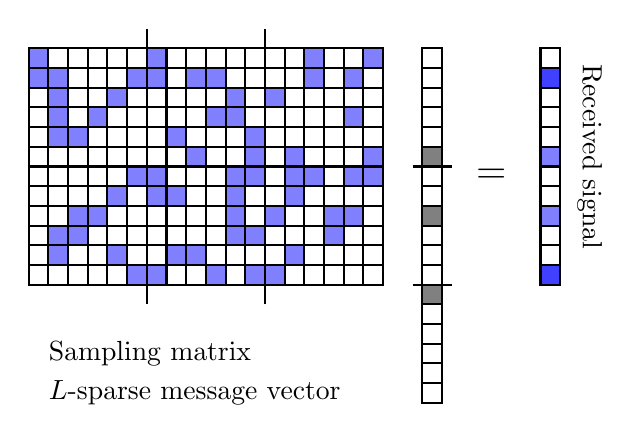
\begin{tikzpicture}
[draw=black, line width=0.75pt,
entry0/.style={rectangle, draw, fill=white, inner sep=0pt, minimum size=2.5mm},
entry1/.style={rectangle, draw, fill=blue!50, inner sep=0pt, minimum size=2.5mm},
symbol0/.style={rectangle, draw, fill=white, inner sep=0pt, minimum size=2.5mm},
symbol1/.style={rectangle, draw, fill=gray, inner sep=0pt, minimum size=2.5mm},
signal0/.style={rectangle, draw, fill=white, inner sep=0pt, minimum size=2.5mm},
signal1/.style={rectangle, draw, fill=blue!50, inner sep=0pt, minimum size=2.5mm},
signal2/.style={rectangle, draw, fill=blue!75, inner sep=0pt, minimum size=2.5mm}]

\node[entry0] (m0600) at (1.50,0) {};
\node[entry0] (m0700) at (1.75,0) {};
\node[entry0] (m0800) at (2.00,0) {};
\node[entry0] (m0900) at (2.25,0) {};
\node[entry0] (m1000) at (2.50,0) {};
\node[entry1] (m1100) at (2.75,0) {};
\node[entry1] (m1200) at (3.00,0) {};
\node[entry0] (m1300) at (3.25,0) {};
\node[entry0] (m1400) at (3.50,0) {};
\node[entry1] (m1500) at (3.75,0) {};
\node[entry0] (m1600) at (4.00,0) {};
\node[entry1] (m1700) at (4.25,0) {};
\node[entry1] (m1800) at (4.50,0) {};
\node[entry0] (m1900) at (4.75,0) {};
\node[entry0] (m2000) at (5.00,0) {};
\node[entry0] (m2100) at (5.25,0) {};
\node[entry0] (m2200) at (5.50,0) {};
\node[entry0] (m2300) at (5.75,0) {};

\node[entry0] (m0601) at (1.50,0.25) {};
\node[entry1] (m0701) at (1.75,0.25) {};
\node[entry0] (m0801) at (2.00,0.25) {};
\node[entry0] (m0901) at (2.25,0.25) {};
\node[entry1] (m1001) at (2.50,0.25) {};
\node[entry0] (m1101) at (2.75,0.25) {};
\node[entry0] (m1201) at (3.00,0.25) {};
\node[entry1] (m1301) at (3.25,0.25) {};
\node[entry1] (m1401) at (3.50,0.25) {};
\node[entry0] (m1501) at (3.75,0.25) {};
\node[entry0] (m1601) at (4.00,0.25) {};
\node[entry0] (m1701) at (4.25,0.25) {};
\node[entry0] (m1801) at (4.50,0.25) {};
\node[entry1] (m1901) at (4.75,0.25) {};
\node[entry0] (m2001) at (5.00,0.25) {};
\node[entry0] (m2101) at (5.25,0.25) {};
\node[entry0] (m2201) at (5.50,0.25) {};
\node[entry0] (m2301) at (5.75,0.25) {};

\node[entry0] (m0602) at (1.50,0.50) {};
\node[entry1] (m0702) at (1.75,0.50) {};
\node[entry1] (m0802) at (2.00,0.50) {};
\node[entry0] (m0902) at (2.25,0.50) {};
\node[entry0] (m1002) at (2.50,0.50) {};
\node[entry0] (m1102) at (2.75,0.50) {};
\node[entry0] (m1202) at (3.00,0.50) {};
\node[entry0] (m1302) at (3.25,0.50) {};
\node[entry0] (m1402) at (3.50,0.50) {};
\node[entry0] (m1502) at (3.75,0.50) {};
\node[entry1] (m1602) at (4.00,0.50) {};
\node[entry1] (m1702) at (4.25,0.50) {};
\node[entry0] (m1802) at (4.50,0.50) {};
\node[entry0] (m1902) at (4.75,0.50) {};
\node[entry0] (m2002) at (5.00,0.50) {};
\node[entry1] (m2102) at (5.25,0.50) {};
\node[entry0] (m2202) at (5.50,0.50) {};
\node[entry0] (m2302) at (5.75,0.50) {};

\node[entry0] (m0603) at (1.50,0.75) {};
\node[entry0] (m0703) at (1.75,0.75) {};
\node[entry1] (m0803) at (2.00,0.75) {};
\node[entry1] (m0903) at (2.25,0.75) {};
\node[entry0] (m1003) at (2.50,0.75) {};
\node[entry0] (m1103) at (2.75,0.75) {};
\node[entry0] (m1203) at (3.00,0.75) {};
\node[entry0] (m1303) at (3.25,0.75) {};
\node[entry0] (m1403) at (3.50,0.75) {};
\node[entry0] (m1503) at (3.75,0.75) {};
\node[entry1] (m1603) at (4.00,0.75) {};
\node[entry0] (m1703) at (4.25,0.75) {};
\node[entry1] (m1803) at (4.50,0.75) {};
\node[entry0] (m1903) at (4.75,0.75) {};
\node[entry0] (m2003) at (5.00,0.75) {};
\node[entry1] (m2103) at (5.25,0.75) {};
\node[entry1] (m2203) at (5.50,0.75) {};
\node[entry0] (m2303) at (5.75,0.75) {};

\node[entry0] (m0604) at (1.50,1.00) {};
\node[entry0] (m0704) at (1.75,1.00) {};
\node[entry0] (m0804) at (2.00,1.00) {};
\node[entry0] (m0904) at (2.25,1.00) {};
\node[entry1] (m1004) at (2.50,1.00) {};
\node[entry0] (m1104) at (2.75,1.00) {};
\node[entry1] (m1204) at (3.00,1.00) {};
\node[entry1] (m1304) at (3.25,1.00) {};
\node[entry0] (m1404) at (3.50,1.00) {};
\node[entry0] (m1504) at (3.75,1.00) {};
\node[entry1] (m1604) at (4.00,1.00) {};
\node[entry0] (m1704) at (4.25,1.00) {};
\node[entry0] (m1804) at (4.50,1.00) {};
\node[entry1] (m1904) at (4.75,1.00) {};
\node[entry0] (m2004) at (5.00,1.00) {};
\node[entry0] (m2104) at (5.25,1.00) {};
\node[entry0] (m2204) at (5.50,1.00) {};
\node[entry0] (m2304) at (5.75,1.00) {};

\node[entry0] (m0605) at (1.50,1.25) {};
\node[entry0] (m0705) at (1.75,1.25) {};
\node[entry0] (m0805) at (2.00,1.25) {};
\node[entry0] (m0905) at (2.25,1.25) {};
\node[entry0] (m1005) at (2.50,1.25) {};
\node[entry1] (m1105) at (2.75,1.25) {};
\node[entry1] (m1205) at (3.00,1.25) {};
\node[entry0] (m1305) at (3.25,1.25) {};
\node[entry0] (m1405) at (3.50,1.25) {};
\node[entry0] (m1505) at (3.75,1.25) {};
\node[entry1] (m1605) at (4.00,1.25) {};
\node[entry1] (m1705) at (4.25,1.25) {};
\node[entry0] (m1805) at (4.50,1.25) {};
\node[entry1] (m1905) at (4.75,1.25) {};
\node[entry1] (m2005) at (5.00,1.25) {};
\node[entry0] (m2105) at (5.25,1.25) {};
\node[entry1] (m2205) at (5.50,1.25) {};
\node[entry1] (m2305) at (5.75,1.25) {};

\node[entry0] (m0606) at (1.50,1.50) {};
\node[entry0] (m0706) at (1.75,1.50) {};
\node[entry0] (m0806) at (2.00,1.50) {};
\node[entry0] (m0906) at (2.25,1.50) {};
\node[entry0] (m1006) at (2.50,1.50) {};
\node[entry0] (m1106) at (2.75,1.50) {};
\node[entry0] (m1206) at (3.00,1.50) {};
\node[entry0] (m1306) at (3.25,1.50) {};
\node[entry1] (m1406) at (3.50,1.50) {};
\node[entry0] (m1506) at (3.75,1.50) {};
\node[entry0] (m1606) at (4.00,1.50) {};
\node[entry1] (m1706) at (4.25,1.50) {};
\node[entry0] (m1806) at (4.50,1.50) {};
\node[entry1] (m1906) at (4.75,1.50) {};
\node[entry0] (m2006) at (5.00,1.50) {};
\node[entry0] (m2106) at (5.25,1.50) {};
\node[entry0] (m2206) at (5.50,1.50) {};
\node[entry1] (m2306) at (5.75,1.50) {};

\node[entry0] (m0607) at (1.50,1.75) {};
\node[entry1] (m0707) at (1.75,1.75) {};
\node[entry1] (m0807) at (2.00,1.75) {};
\node[entry0] (m0907) at (2.25,1.75) {};
\node[entry0] (m1007) at (2.50,1.75) {};
\node[entry0] (m1107) at (2.75,1.75) {};
\node[entry0] (m1207) at (3.00,1.75) {};
\node[entry1] (m1307) at (3.25,1.75) {};
\node[entry0] (m1407) at (3.50,1.75) {};
\node[entry0] (m1507) at (3.75,1.75) {};
\node[entry0] (m1607) at (4.00,1.75) {};
\node[entry1] (m1707) at (4.25,1.75) {};
\node[entry0] (m1807) at (4.50,1.75) {};
\node[entry0] (m1907) at (4.75,1.75) {};
\node[entry0] (m2007) at (5.00,1.75) {};
\node[entry0] (m2107) at (5.25,1.75) {};
\node[entry0] (m2207) at (5.50,1.75) {};
\node[entry0] (m2307) at (5.75,1.75) {};

\node[entry0] (m0608) at (1.50,2.00) {};
\node[entry1] (m0708) at (1.75,2.00) {};
\node[entry0] (m0808) at (2.00,2.00) {};
\node[entry1] (m0908) at (2.25,2.00) {};
\node[entry0] (m1008) at (2.50,2.00) {};
\node[entry0] (m1108) at (2.75,2.00) {};
\node[entry0] (m1208) at (3.00,2.00) {};
\node[entry0] (m1308) at (3.25,2.00) {};
\node[entry0] (m1408) at (3.50,2.00) {};
\node[entry1] (m1508) at (3.75,2.00) {};
\node[entry1] (m1608) at (4.00,2.00) {};
\node[entry0] (m1708) at (4.25,2.00) {};
\node[entry0] (m1808) at (4.50,2.00) {};
\node[entry0] (m1908) at (4.75,2.00) {};
\node[entry0] (m2008) at (5.00,2.00) {};
\node[entry0] (m2108) at (5.25,2.00) {};
\node[entry1] (m2208) at (5.50,2.00) {};
\node[entry0] (m2308) at (5.75,2.00) {};

\node[entry0] (m0609) at (1.50,2.25) {};
\node[entry1] (m0709) at (1.75,2.25) {};
\node[entry0] (m0809) at (2.00,2.25) {};
\node[entry0] (m0909) at (2.25,2.25) {};
\node[entry1] (m1009) at (2.50,2.25) {};
\node[entry0] (m1109) at (2.75,2.25) {};
\node[entry0] (m1209) at (3.00,2.25) {};
\node[entry0] (m1309) at (3.25,2.25) {};
\node[entry0] (m1409) at (3.50,2.25) {};
\node[entry0] (m1509) at (3.75,2.25) {};
\node[entry1] (m1609) at (4.00,2.25) {};
\node[entry0] (m1709) at (4.25,2.25) {};
\node[entry1] (m1809) at (4.50,2.25) {};
\node[entry0] (m1909) at (4.75,2.25) {};
\node[entry0] (m2009) at (5.00,2.25) {};
\node[entry0] (m2109) at (5.25,2.25) {};
\node[entry0] (m2209) at (5.50,2.25) {};
\node[entry0] (m2309) at (5.75,2.25) {};

\node[entry1] (m0610) at (1.50,2.50) {};
\node[entry1] (m0710) at (1.75,2.50) {};
\node[entry0] (m0810) at (2.00,2.50) {};
\node[entry0] (m0910) at (2.25,2.50) {};
\node[entry0] (m1010) at (2.50,2.50) {};
\node[entry1] (m1110) at (2.75,2.50) {};
\node[entry1] (m1210) at (3.00,2.50) {};
\node[entry0] (m1310) at (3.25,2.50) {};
\node[entry1] (m1410) at (3.50,2.50) {};
\node[entry1] (m1510) at (3.75,2.50) {};
\node[entry0] (m1610) at (4.00,2.50) {};
\node[entry0] (m1710) at (4.25,2.50) {};
\node[entry0] (m1810) at (4.50,2.50) {};
\node[entry0] (m1910) at (4.75,2.50) {};
\node[entry1] (m2010) at (5.00,2.50) {};
\node[entry0] (m2110) at (5.25,2.50) {};
\node[entry1] (m2210) at (5.50,2.50) {};
\node[entry0] (m2310) at (5.75,2.50) {};

\node[entry1] (m0611) at (1.50,2.75) {};
\node[entry0] (m0711) at (1.75,2.75) {};
\node[entry0] (m0811) at (2.00,2.75) {};
\node[entry0] (m0911) at (2.25,2.75) {};
\node[entry0] (m1011) at (2.50,2.75) {};
\node[entry0] (m1111) at (2.75,2.75) {};
\node[entry1] (m1211) at (3.00,2.75) {};
\node[entry0] (m1311) at (3.25,2.75) {};
\node[entry0] (m1411) at (3.50,2.75) {};
\node[entry0] (m1511) at (3.75,2.75) {};
\node[entry0] (m1611) at (4.00,2.75) {};
\node[entry0] (m1711) at (4.25,2.75) {};
\node[entry0] (m1811) at (4.50,2.75) {};
\node[entry0] (m1911) at (4.75,2.75) {};
\node[entry1] (m2011) at (5.00,2.75) {};
\node[entry0] (m2111) at (5.25,2.75) {};
\node[entry0] (m2211) at (5.50,2.75) {};
\node[entry1] (m2311) at (5.75,2.75) {};

\draw (2.875,-0.375) -- (2.875,3.125);
\draw (4.375,-0.375) -- (4.375,3.125);

\node[symbol0] (s07) at (6.5,-1.50) {};
\node[symbol0] (s08) at (6.5,-1.25) {};
\node[symbol0] (s09) at (6.5,-1.00) {};
\node[symbol0] (s10) at (6.5,-0.75) {};
\node[symbol0] (s11) at (6.5,-0.50) {};
\node[symbol1] (s12) at (6.5,-0.25) {};
\draw (6.25,-0.125) -- (6.75,-0.125);
\node[symbol0] (s13) at (6.5,0) {};
\node[symbol0] (s14) at (6.5,0.25) {};
\node[symbol0] (s15) at (6.5,0.50) {};
\node[symbol1] (s16) at (6.5,0.75) {};
\node[symbol0] (s17) at (6.5,1.00) {};
\node[symbol0] (s18) at (6.5,1.25) {};
\draw (6.25,1.375) -- (6.75,1.375);
\node[symbol1] (s19) at (6.5,1.50) {};
\node[symbol0] (s20) at (6.5,1.75) {};
\node[symbol0] (s21) at (6.5,2.00) {};
\node[symbol0] (s22) at (6.5,2.25) {};
\node[symbol0] (s23) at (6.5,2.50) {};
\node[symbol0] (s24) at (6.5,2.75) {};

\node (equal) at (7.25,1.25) {\Large =};

\node[signal2] (y00) at (8,0) {};
\node[signal0] (y01) at (8,0.25) {};
\node[signal0] (y02) at (8,0.50) {};
\node[signal1] (y03) at (8,0.75) {};
\node[signal0] (y04) at (8,1.00) {};
\node[signal0] (y05) at (8,1.25) {};
\node[signal1] (y06) at (8,1.50) {};
\node[signal0] (y07) at (8,1.75) {};
\node[signal0] (y08) at (8,2.00) {};
\node[signal0] (y09) at (8,2.25) {};
\node[signal2] (y10) at (8,2.50) {};
\node[signal0] (y11) at (8,2.75) {};

\node[anchor=west] (samplingmatrix) at (1.5,-1) {Sampling matrix};
\node[anchor=west] (vector) at (1.5,-1.5) {$L$-sparse message vector};
\node[rotate=-90] (receivedsignal) at (8.5,1.5) {Received signal};
\end{tikzpicture}

\end{center}
\begin{itemize}
\item Complexity reduction due to narrower $\Am$
\item Use full sensing matrix $\Am$
\item Decode inner code with low-complexity AMP
\end{itemize}
%\myfootnote{\tiny
%A. Fengler, P. Jung, and G. Caire.
%\emph{SPARCs and AMP for Unsourced Random Access}.
%ISIT 2019}
\end{frame}

% % % % % % % % % % % % % % % % % % % %

\begin{frame}
\frametitle{CCS -- Approximate Message Passing}
% % % % %
\begin{block}{Governing Equations}
\begin{itemize}
\item AMP algorithm iterates through
\begin{align*}
\zv^{(t)} &= \yv - \Am \Dm \etav_t \big( \rv^{(t)} \big)
+ \underbrace{\frac{\zv^{(t-1)}}{n} \operatorname{div} \mathbf{D} \etav_t \big( \rv^{(t)} \big)}_{\text{Onsager correction}} \\
\rv^{(t+1)} &= \Am^{\transpose} \zv^{(t)} + \Dm
\underbrace{\etav_t \big( \rv^{(t)} \big)}_{\text{Denoiser}}
\end{align*}
\textcolor{gray}{Initial conditions $\zv^{(0)} = \zerov$ and $\etav_0 \left( \rv^{(0)} \right) = \zerov$}
\item Application falls within framework for non-separable functions
\end{itemize}
\end{block}
% % % % %
\vfill
% % % % %
\begin{exampleblock}{Task}
\begin{itemize}
\item Define denoiser and compute Onsager correction term
\end{itemize}
\end{exampleblock}
\end{frame}

% % % % % % % % % % % % % % % % % % % %

\begin{frame}
\frametitle{Marginal Posterior Mean Estimate (PME)}
% % % % %
\begin{block}{Proposed Denoiser (Fengler, Jung, and Caire)}
\begin{itemize}
\item State estimate based on Gaussian model
\begin{equation*}
\begin{split}
\hat{s}^{\mathrm{OR}} & \left( q, r, \tau \right)
= \mathbb{E} \left[ s \middle| \sqrt{P_{\ell}} s + \tau \zeta = r \right] \\
%&= \frac{0 \cdot \Pr (s = 0) f \left( \frac{r}{\tau} \right) + 1 \cdot \Pr (s = 1) f \left( \frac{r - d_{\ell}}{\tau} \right)}{\Pr (s = 0) f \left( \frac{r}{\tau} \right) + \Pr (s = 1) f \left( \frac{r - d_{\ell}}{\tau} \right)} \\
&= \frac{q \exp \left( - \frac{ \left( r - \sqrt{P_{\ell}} \right)^2}{2 \tau^2} \right)}
{(1-q) \exp \left( -\frac{r^2}{2 \tau^2} \right)
+ q \exp \left( - \frac{ \left( r - \sqrt{P_{\ell}} \right)^2}{2 \tau^2} \right)}
\end{split}
\end{equation*}
with (essentially) uninformative prior $q = K/m$ fixed
\item $\etav_t \left( \mathbf{r}^{(t)} \right)$ is aggregate of PME values
\item $\tau_t$ is obtained from state evolution or $\tau_t^2 = {\| \mathbf{z}^{(t)} \|^2}/{n}$
\end{itemize}
\end{block}
\end{frame}

% % % % % % % % % % % % % % % % % % % %

\begin{frame}
\frametitle{Performance of CCS-AMP versus Previous Schemes}
% % % % %
\begin{center}
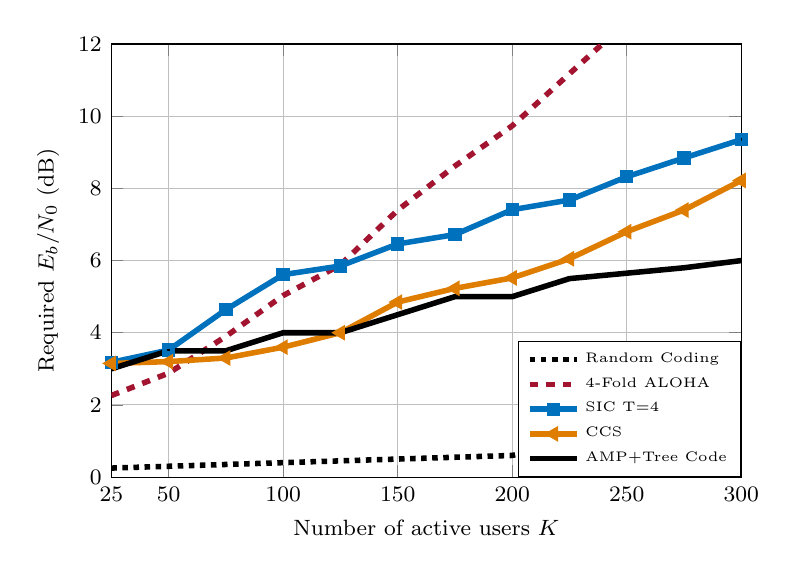
\begin{tikzpicture}
\definecolor{mycolor1}{rgb}{0.63529,0.07843,0.18431}%
\definecolor{mycolor2}{rgb}{0.00000,0.44706,0.74118}%
\definecolor{mycolor3}{rgb}{0.00000,0.49804,0.00000}%
\definecolor{mycolor4}{rgb}{0.87059,0.49020,0.00000}%
\definecolor{mycolor5}{rgb}{0.00000,0.44700,0.74100}%
\definecolor{mycolor6}{rgb}{0.74902,0.00000,0.74902}%

\begin{axis}[%
font=\footnotesize,
width=8cm,
height=5.5cm,
scale only axis,
xmin=25,
xmax=300,
xtick = {25,50,100,...,300},
xlabel={Number of active users $K$},
xmajorgrids,
ymin=0,
ymax=12,
ytick = {0,2,...,12},
ylabel={Required $E_b/N_0$ (dB)},
ylabel near ticks,
ymajorgrids,
legend style={font=\tiny, at={(1,0)},anchor=south east, draw=black,fill=white,legend cell align=left}
]

\addplot [color=black,dotted,line width=2.0pt]
  table[row sep=crcr]{
 25	0.25\\
50	0.3\\
75	0.35\\
100	0.4\\
125	0.45\\
150	0.5\\
175	0.55\\
200	0.6\\
225	0.95\\
250	1.25\\
275	1.55\\
300	1.8\\
};
\addlegendentry{Random Coding};

\addplot [color=mycolor1,dashed,line width=2.0pt]
  table[row sep=crcr]{25	2.26\\
50	2.88\\
75	3.9\\
100	5.03\\
125	5.8798\\
150	7.3954\\
175	8.6199\\
200	9.7328\\
225	11.1761\\
250	12.6127\\
275	13.3907\\
300	14.9116\\
};
\addlegendentry{4-Fold ALOHA};

%\addplot [color=mycolor3,solid,line width=2.0pt]
  %table[row sep=crcr]{25	7.5\\
%35	7.3\\
%50	8.75\\
%100	11.7\\
%150	14.5\\
%200	18\\
%250	21\\
%300	23\\
%};
%\addlegendentry{OP-Exact};

\addplot [color=mycolor2,solid,line width=2.0pt,mark size=1.4pt,mark=square,mark options={solid}]
  table[row sep=crcr]{25	3.18\\
50	3.52\\
75	4.64\\
100	5.61\\
125	5.85\\
150	6.46\\
175	6.72\\
200	7.41\\
225	7.6772\\
250	8.3217\\
275	8.8428\\
300	9.352\\
};
\addlegendentry{SIC T=4};

\addplot [color=mycolor4,solid,line width=2.0pt,mark size=1.3pt,mark=triangle,mark options={solid,rotate=90}]
  table[row sep=crcr]{
  25  3.15\\
50	3.2\\
75	3.3\\
100	3.6\\
125	4\\
150	4.85\\
175	5.23\\
200	5.52\\
225	6.05\\
250	6.8\\
275	7.4\\
300	8.22\\
};
\addlegendentry{CCS};

\addplot [color=black,solid,line width=2.0pt]
  table[row sep=crcr]{
25	3\\
50	3.5\\
75  3.5\\
100	4\\
125	4\\
150 4.5\\
175 5\\
200	5\\
225 5.5
250	5.8\\
275 5.8\\
300	6\\
};
\addlegendentry{AMP+Tree Code};

%\addplot [color=mycolor3,solid,line width=2.0pt,mark size=1.4pt,mark=square,mark options={solid}]
%  table[row sep=crcr]{
%  25  2\\
%50	2.1\\
%75	2.2\\
%100	2.41\\
%125	2.57\\
%150	2.81\\
%175	3\\
%200 3.4\\
%225 3.88\\
%250 4.36\\
%275 4.87\\
%300 5.35\\
%};
%\addlegendentry{Sparse IDMA};
%\node[] at (axis cs: 300,5.15) {\scriptsize \textcolor{red}{O}};
%\node[] at (axis cs: 275,4.69) {\scriptsize \textcolor{red}{O}};
%\node[] at (axis cs: 225,3.7) {\scriptsize \textcolor{red}{O}};

%\addplot [color=violet,solid,line width=2.0pt]
%  table[row sep=crcr]{
%10 0.3801\\
%20 0.5939\\
%30 0.8524\\
%40 0.9949\\
%50 1.1553\\
%60 1.3246\\
%70 1.5474\\
%80 1.7167\\
%90 1.8682\\
%100 2.0554\\
%110 2.2247\\
%120 2.3762\\
%130 2.5811\\
%140 2.7950\\
%150 2.9999\\
%160 3.1425\\
%170 3.3475\\
%180 3.5168\\
%190 3.7128\\
%200 3.8911\\
%210 4.0425\\
%220 4.2742\\
%230 4.5505\\
%240 4.7554\\
%250 4.9158\\
%260 5.0762\\
%270 5.2010\\
%280 5.3168\\
%290 5.4059\\
%300 5.4951\\
%310 5.5663\\
%320 5.6376\\
%330 5.6911\\
%340 5.7357\\
%350 5.7624\\
%360 5.7802\\
%370 5.8069\\
%380 5.8248\\
%390 5.8515\\
%400 5.9050\\
%410 6.0119\\
%420 6.1634\\
%430 6.6000\\
%};
%\addlegendentry{Polar Codes};

\end{axis}


\end{tikzpicture}

\end{center}
\end{frame}

% % % % % % % % % % % % % % % % % % % %

\begin{frame}
\frametitle{Incorporating Lessons from Enhanced CCS}
% % % % %
\begin{itemize}
\item Integrate outer code structure into inner decoding
\end{itemize}
\begin{center}
\begin{tikzpicture}
[font=\footnotesize, draw=black, line width=0.75pt,>=stealth',
sub0/.style={rectangle, draw, inner sep=0pt, minimum width=10mm, minimum height=2.5mm},
parity/.style={rectangle, draw, fill=teal!75, inner sep=0pt, minimum size=2.5mm}]

%\node (cs1) at (0.00,6.125) {Slot~1};
%\node (cs2) at (2.50,6.125) {Slot~2};
%\node (cs3) at (5.00,6.125) {Slot~3};

\foreach \v in {0.00,2.50,5.00} {
  \draw[->, line width=1pt]  (\v,3.875) -- (\v,3.375);
  \draw[->, line width=1pt]  (\v,5.75) -- (\v,5.25);
  \draw[dotted, line width=1pt, draw=gray]  (\v-0.25,5.65) -- (\v,5.25);
  \draw[dotted, line width=1pt, draw=gray]  (\v-0.125,5.7) -- (\v,5.25);
  \draw[dotted, line width=1pt, draw=gray]  (\v+0.125,5.7) -- (\v,5.25);
  \draw[dotted, line width=1pt, draw=gray]  (\v+0.25,5.65) -- (\v,5.25);
}

\foreach \v in {0.00} {
  \draw[line width=1pt] (\v-0.5,5) -- (\v-0.625,5) -- (\v-0.625,4.5) -- (\v-0.5,4.5);
  \draw[line width=1pt] (\v+0.375,5) -- (\v+0.5,5) -- (\v+0.5,4.5) -- (\v+0.375,4.5);
  \draw[line width=1pt] (\v+0.575,5) -- (\v+0.575,3.875) -- (\v+0.695,3.875) -- (\v+0.695,5) -- (\v+0.575,5);
}

\foreach \v in {2.50,5.00} {
  \draw[line width=1pt] (\v-0.275,5) -- (\v-0.4,5) -- (\v-0.4,4.5) -- (\v-0.275,4.5);
  \draw[line width=1pt] (\v+0.15,5) -- (\v+0.275,5) -- (\v+0.275,4.5) -- (\v+0.15,4.5);
  \draw[line width=1pt] (\v+0.35,5) -- (\v+0.35,4.325) -- (\v+0.47,4.325) -- (\v+0.47,5) -- (\v+0.35,5);
}

\foreach \p/\c in {3.00/1, 2.625/2, 2.25/3, 1.875/4} {
  \node[parity] (subcs00c\c) at (-0.375,\p) {};
  \node[parity] (subcs01c\c) at (-0.125,\p) {};
  \node[parity] (subcs02c\c) at (0.125,\p) {};
  \node[parity] (subcs02c\c) at (0.375,\p) {};

  \node[parity] (subcs03c\c) at (2.125,\p) {};
  \node[parity] (subcs04c\c) at (2.375,\p) {};
  \node[parity] (subcs05c\c) at (2.625,\p) {};
  \node[parity] (subcs05c\c) at (2.875,\p) {};

  \node[parity] (subcs06c\c) at (4.625,\p) {};
  \node[parity] (subcs07c\c) at (4.875,\p) {};
  \node[parity] (subcs08c\c) at (5.125,\p) {};
  \node[parity] (subcs08c\c) at (5.375,\p) {};
}



\node (list1) at (0.00,1.25) {List~1};
\node (list2) at (2.50,1.25) {List~2};
\node (list3) at (5.00,1.25) {List~3};

\draw [line width=1.5pt,color=purple,->] plot[smooth, tension=.5] coordinates {(0.5,1.25) (1.25,1.75) (1.375,4) (1.875,4.75)};
\draw [line width=1.5pt,color=purple,->] plot[smooth, tension=.5] coordinates {(3.0,1.25) (3.75,1.75) (3.875,4) (4.375,4.75)};
\draw [line width=1.5pt,color=purple,dashed] plot[smooth, tension=.5] coordinates {(5.5,1.25) (6.25,1.75) (6.375,4.25)};

\node[rotate=90] (prune1) at (1.0625,3) {column pruning};
\node[rotate=90] (prune2) at (3.5625,3) {column pruning};
\node[rotate=90] (prune3) at (6.0625,3) {column pruning};
\end{tikzpicture}

\end{center}
\begin{alertblock}{Challenges}
\begin{itemize}
\item CCS-AMP inner decoding is not a sequence of hard decisions
\item List size for CCS-AMP is effective length of index vector
\end{itemize}
\end{alertblock}
\myfootnote{\tiny
V.~K. Amalladinne, A.~K. Pradhan, C. Rush, J.-F. Chamberland, K.~R. Narayanan.
\emph{On approximate message passing for unsourced access with coded compressed sensing.}
ISIT 2020}

\end{frame}

% % % % % % % % % % % % % % % % % % % %

\begin{frame}
\frametitle{Redesigning Outer Code}
% % % % %
\begin{block}{Properties of Original Outer Code}
\begin{itemize}
\item Aimed at stitching message fragments together
\item Works on short lists of $K$ fragments
\item Parities allocated to control growth and complexity
\end{itemize}
\end{block}
\begin{center}
\begin{tikzpicture}[
  font=\footnotesize, >=stealth', line width=0.75pt,
  infobits0/.style={rectangle, minimum height=4mm, minimum width=10mm, draw=black, fill=gray!10, rounded corners},
  infobits/.style={rectangle, minimum height=4mm, minimum width=6mm, draw=black, fill=gray!10, rounded corners},
  paritybits/.style={rectangle, minimum height=4mm, minimum width=4mm, draw=black, fill=gray!40, rounded corners},
  dot/.style={circle, minimum width=2pt, draw=black, inner sep=0pt}
]

\node[infobits0] (vb0) at (0,1.5) {};
\node[infobits] (vb1) at (0.8,1.5) {};
\node[paritybits] (vp1) at (1.3,0) {};
\node[infobits] (vb2) at (1.8,1.5) {};
\node[paritybits] (vp2) at (2.3,0) {};
\node[infobits] (vb3) at (2.8,1.5) {};
\node[paritybits] (vp3) at (3.3,0) {};
\node[infobits] (vb4) at (3.8,1.5) {};
\node[paritybits] (vp4) at (4.3,0) {};
\node[infobits] (vb5) at (4.8,1.5) {};
\node[paritybits] (vp5) at (5.3,0) {};

\node[dot] (vb0dot) at (0.0,1.2) {};
\node[dot] (vb1dot) at (0.8,1.2) {};
\node[dot] (vp1dot) at (1.3,0.3) {}
  edge[-,dashed,draw=lightgray] (vb0dot);
\node[dot] (vb2dot) at (1.8,1.2) {};
\node[dot] (vp2dot) at (2.3,0.3) {}
  edge[-,dashed,draw=lightgray] (vb0dot)
  edge[-,dashed,draw=lightgray] (vb1dot);
\node[dot] (vb3dot) at (2.8,1.2) {};
\node[dot] (vp3dot) at (3.3,0.3) {}
  edge[-,dashed,draw=lightgray] (vb0dot)
  edge[-,dashed,draw=lightgray] (vb1dot)
  edge[-,dashed,draw=lightgray] (vb2dot);
\node[dot] (vb4dot) at (3.8,1.2) {};
\node[dot] (vp4dot) at (4.3,0.3) {}
  edge[-] (vb0dot)
  edge[-] (vb1dot)
  edge[-] (vb2dot)
  edge[-] (vb3dot);
\node[dot] (vb5dot) at (4.8,1.2) {};
\node[dot] (vp5dot) at (5.3,0.3) {}
  edge[-,dashed,draw=lightgray] (vb0dot)
  edge[-,dashed,draw=lightgray] (vb1dot)
  edge[-,dashed,draw=lightgray] (vb2dot)
  edge[-,dashed,draw=lightgray] (vb3dot)
  edge[-,dashed,draw=lightgray] (vb4dot);

\foreach \x in {-0.5,0.5,1.5,2.5,3.5,4.5,5.5} {
    \draw[dotted] (\x,-0.5) -- (\x,2);
}
\end{tikzpicture}

\end{center}
\begin{block}{Challenges to Integrate into AMP}
\begin{enumerate}
\item Must compute beliefs for all possible $2^v$ fragments
\item Must provide pertinent information to inner AMP decoder
\item Should maintain ability to stitch outer code
\end{enumerate}
\end{block}
\end{frame}

% % % % % % % % % % % % % % % % % % % %

\begin{frame}
\frametitle{Factor Graph Interpretation of Outer Code}
% % % % %
\begin{center}
\scalebox{0.9}{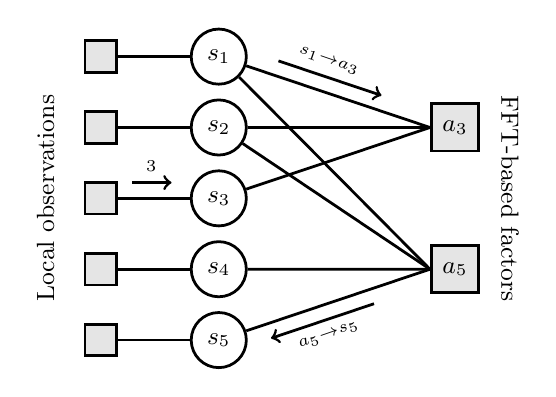
\begin{tikzpicture}
  [
  font=\small, line width=1pt, draw=black,
  check/.style={rectangle, minimum height=6mm, minimum width=6mm, draw=black, fill=gray!20},
  trivialcheck/.style={rectangle, minimum height=4mm, minimum width=4mm, draw=black, fill=gray!20},
  section/.style={circle, minimum size=7mm, draw=black}
  ]

\foreach \m in {1,2,3,4,5} {
  \node[section] (s\m) at (0,2.7-0.9*\m) {$s_{\m}$};
}

\foreach \t in {1,2,3,4,5} {
  \node[trivialcheck] (t\t) at (-1.5,2.7-0.9*\t) {}
    edge (s\t);
}

\node[check] (a3) at (3,0.9) {$a_3$};
\node[check] (a5) at (3,-0.9) {$a_5$};

\node[rotate=90] (variable) at (-2.2,0) {Local observations};
\node[rotate=-90] (check) at (3.7,0) {FFT-based factors};

\draw (s1) -- (a3.west);
\draw (s2) -- (a3.west);
\draw (s3) -- (a3.west);
\draw (s1) -- (a5.west);
\draw (s2) -- (a5.west);
\draw (s4) -- (a5.west);
\draw (s5) -- (a5.west);

\draw[shorten <=0.8cm,shorten >=0.65cm,->] (s1)++(0,0.2cm) -- node[above,rotate=-19] {$\muv_{s_1 \to a_3}$} ([yshift=0.2cm]a3.west);
\draw[shorten <=0.7cm,shorten >=0.75cm,<-] (s5)++(0,-0.2cm) -- node[below,rotate=19] {$\muv_{a_5 \to s_5}$} ([yshift=-0.2cm]a5.west);
\draw[shorten <=0.4cm,shorten >=0.4cm,->] (t3)++(0,0.2cm) -- node[above] {$\lambdav_3$} (-0.2,0.2cm);

\end{tikzpicture}
}
\end{center}
\begin{itemize}
\item Outer code with circular convolution structure
\end{itemize}
\begin{equation*}
\muv_{a_p \to s_{\ell}} \left( \left[ \hat{\vv}(\ell) \right]_2 \right)
\propto
\frac{1}{\left\| \gv_{\ell, p}^{(g)} \right\|_0}
\left( \operatorname{FFT}^{-1} \left( \prod_{s_j \in N(a_p) \setminus s_{\ell}} \operatorname{FFT} \left( \lambdav_{j,p} \right) \right) \right) (g)
\end{equation*}
\end{frame}

% % % % % % % % % % % % % % % % % % % %

\begin{frame}
\frametitle{Outer Code and Mixing}
% % % % %
\begin{center}
\scalebox{0.9}{\begin{tikzpicture}[
  font=\small, >=stealth', line width=0.75pt,
  infobits/.style={rectangle, minimum height=6.5mm, minimum width=10mm, draw=black, fill=gray!20, rounded corners},
  paritybits/.style={rectangle, minimum height=6.5mm, minimum width=10mm, draw=black, fill=gray!20, rounded corners},
  impossibleblocks/.style={rectangle, minimum height=6.5mm, minimum width=10mm, draw=black, fill=none, rounded corners}
]

\node[infobits] (v10) at (0,0) {0};
\node[impossibleblocks] (v11) at (0,1) {{1}};
\node[infobits] (v12) at (0,2) {2};
\node[impossibleblocks] (v13) at (0,3) {{3}};

\node[impossibleblocks] (v20) at (3,0) {{0}};
\node[infobits] (v21) at (3,1) {1};
\node[infobits] (v22) at (3,2) {2};
\node[impossibleblocks] (v23) at (3,3) {{3}};

\node[paritybits] (v30) at (6,0) {{0}};
\node[paritybits] (v31) at (6,1) {{1}};
\node[paritybits] (v32) at (6,2) {2};
\node[paritybits] (v33) at (6,3) {3};

\foreach \y/\ya in {0/-0.15,1/-0.05,2/0.05,3/0.15}{
    \foreach \yb in {0,1,2,3}{
        \draw[dashed] (0.5,\y+\ya) -- (2.5,\yb+\ya);
    }
}

\foreach \yexit/\yentry in {0/0,1/1,2/2,3/3}{
    \draw[dashed] (3.5,\yexit-0.15) -- (5.5,\yentry-0.15);
}
\foreach \yexit/\yentry in {0/1,1/2,2/3,3/0}{
    \draw[dashed] (3.5,\yexit-0.05) -- (5.5,\yentry-0.05);
}
\foreach \yexit/\yentry in {0/2,1/3,2/0,3/1}{
    \draw[dashed] (3.5,\yexit+0.05) -- (5.5,\yentry+0.05);
}
\foreach \yexit/\yentry in {0/3,1/0,2/1,3/2}{
    \draw[dashed] (3.5,\yexit+0.15) -- (5.5,\yentry+0.15);
}

\draw[line width=1.25pt] (0.5,0-0.15) -- (2.5,1-0.15);
\draw[line width=1.25pt] (0.5,0-0.15) -- (2.5,2-0.15);
\draw[line width=1.25pt] (0.5,2+0.05) -- (2.5,1+0.05);
\draw[line width=1.25pt] (0.5,2+0.05) -- (2.5,2+0.05);

\draw[line width=1.25pt] (3.5,1+0.05) -- (5.5,1+0.05);
\draw[line width=1.25pt] (3.5,1+0.05) -- (5.5,3+0.05);
\draw[line width=1.25pt] (3.5,2-0.15) -- (5.5,2-0.15);
\draw[line width=1.25pt] (3.5,2-0.15) -- (5.5,0-0.15);


\node (w1) at (0,-1) {$\left[ \hat{\vv}(1) \mathbf{G}_{1,3} \right]$};
\node (w2) at (3,-1) {$\left[ \hat{\vv}(2) \mathbf{G}_{2,3} \right]$};
\node (p3) at (6,-1) {$\vv(3)$};

\end{tikzpicture}
}
\end{center}
\begin{itemize}
\item Multiple devices on same graph
\item Parity factor mix concentrated values
\item Suggests triadic outer structure
\end{itemize}
\end{frame}

% % % % % % % % % % % % % % % % % % % %

\begin{frame}
\frametitle{Redesigning Outer Code}
% % % % %
\begin{block}{Solutions to Integrate into AMP}
\begin{itemize}
\item Parity bits are generated over Abelian group amenable to\\
FWHT or FFT
\item Discrimination power proportional to \# parities
\end{itemize}
\end{block}
\begin{center}
\begin{tikzpicture}[
  font=\footnotesize, >=stealth', line width=0.75pt,
  infobits/.style={rectangle, minimum height=4mm, minimum width=10mm, draw=black, fill=gray!10, rounded corners},
  paritybits/.style={rectangle, minimum height=4mm, minimum width=10mm, draw=black, fill=gray!40, rounded corners},
  dot/.style={circle, minimum width=2pt, draw=black, inner sep=0pt}
]

\node[infobits] (vb0) at (0,1) {};
\node[infobits] (vb1) at (1,1) {};
\node[paritybits] (vp2) at (2,0) {};
\node[infobits] (vb3) at (3,1) {};
\node[infobits] (vb4) at (4,1) {};
\node[paritybits] (vp5) at (5,0) {};

\node[dot] (vb0dot) at (0,0.7) {};
\node[dot] (vb1dot) at (1,0.7) {};
\node[dot] (vp2dot) at (2,0.3) {}
  edge[-] (vb0dot)
  edge[-] (vb1dot);
\node[dot] (vb3dot) at (3,0.7) {};
\node[dot] (vb4dot) at (4,0.7) {};
\node[dot] (vp5dot) at (5,0.3) {}
  edge[-] (vb3dot)
  edge[-] (vb4dot);

\foreach \x in {-0.5,0.5,1.5,2.5,3.5,4.5,5.5} {
    \draw[dotted] (\x,-0.5) -- (\x,1.5);
}
\end{tikzpicture}

\end{center}
\begin{block}{New Design Strategy}
\begin{enumerate}
\item Information sections with parity bits interspersed in-between
\item Parity over two blocks (triadic dependencies)
\end{enumerate}
\end{block}
\end{frame}

% % % % % % % % % % % % % % % % % % % %

\begin{frame}
\frametitle{Belief Propagation -- Message Passing Rules}
% % % % %
\begin{center}
\scalebox{0.85}{\begin{tikzpicture}[
  font=\small, >=stealth', line width=0.75pt,
  infobits/.style={rectangle, minimum height=3mm, minimum width=10mm, draw=black, fill=gray!10, rounded corners},
  paritybits/.style={rectangle, minimum height=3mm, minimum width=10mm, draw=black, fill=gray!40, rounded corners}
]

\node[infobits] (vb1) at (1,0) {$\vv(1)$};
\node[infobits] (vb2) at (2,0) {$\vv(2)$};
\node[infobits] (vb4) at (3,0) {$\vv(4)$};
\node[infobits] (vb5) at (4,0) {$\vv(5)$};
\node[infobits] (vb7) at (5,0) {$\vv(7)$};
\node[infobits] (vb8) at (6,0) {$\vv(8)$};
\node[infobits] (vb10) at (7,0) {$\vv(10)$};
\node[infobits] (vb11) at (8,0) {$\vv(11)$};

\node[paritybits] (vp3) at (1.5,-1) {$\vv(3)$};
\node[paritybits] (vp6) at (3.5,-1) {$\vv(6)$};
\node[paritybits] (vp9) at (5.5,-1) {$\vv(9)$};
\node[paritybits] (vp12) at (7.5,-1) {$\vv(12)$};
\node[paritybits] (vp13) at (1.5,1) {$\vv(13)$};
\node[paritybits] (vp14) at (3.5,1) {$\vv(14)$};
\node[paritybits] (vp15) at (5.5,1) {$\vv(15)$};

\node[paritybits] (vp16) at (7.5,1) {$\vv(16)$};

\draw  (vb1.south) edge (vp3);
\draw  (vb2.south) edge (vp3);
\draw  (vb4.south) edge (vp6);
\draw  (vb5.south) edge (vp6);
\draw  (vb7.south) edge (vp9);
\draw  (vb8.south) edge (vp9);
\draw  (vb10.south) edge (vp12);
\draw  (vb11.south) edge (vp12);

\draw  (vb1.north) edge (vp13);
\draw  (vb7.north) edge (vp13);
\draw  (vb2.north) edge (vp14);
\draw  (vb10.north) edge (vp14);
\draw  (vb4.north) edge (vp15);
\draw  (vb8.north) edge (vp15);
\draw  (vb5.north) edge (vp16);
\draw  (vb11.north) edge (vp16);

\end{tikzpicture}
}
\end{center}
\begin{itemize}
\item Message from check node $a_p$ to variable node $s \in N(a_p)$:
\begin{equation*}
\textstyle \muv_{a_p \to s} (k)
= \sum_{\kv_{a_p}: k_p = k} \mathcal{G}_{a_p} \left( \kv_{a_p} \right)
\prod_{s_j \in N(a_p) \setminus s} \muv_{s_j \to a_p} (k_j)
\end{equation*}
\item Message from variable node $s_{\ell}$ to check node $a \in N(s)$:
\begin{equation*}
\textstyle \muv_{s_{\ell} \rightarrow a} (k)
\propto \lambdav_{\ell} (k) \prod_{a_p \in N(s_{\ell}) \setminus a} \muv_{a_p \to s_{\ell}} (k)
\end{equation*}
\item Estimated marginal distribution
\begin{equation*}
\textstyle p_{s_{\ell}} (k) \propto \boldsymbol{\lambda}_{\ell} (k) \prod_{a \in N(s_{\ell})} \boldsymbol{\mu}_{a \to s_{\ell}} (k)
\end{equation*}
\end{itemize}
\end{frame}

% % % % % % % % % % % % % % % % % % % %

\begin{frame}
\frametitle{Approximate Message Passing Algorithm}
% % % % %
\begin{block}{Updated Equations}
AMP two-step algorithm
\begin{align*}
\zv^{(t)} &= \yv - \Am \Dm \etav_t \big( \rv^{(t)} \big)
+ \underbrace{\frac{\zv^{(t-1)}}{n} \operatorname{div} \mathbf{D} \etav_t \big( \rv^{(t)} \big)}_{\text{Correction}} \\
\rv^{(t+1)} &= \Am^{\transpose} \zv^{(t)} + \Dm
\underbrace{\etav_t \big( \rv^{(t)} \big)}_{\text{Denoiser}}
\end{align*}
\textcolor{gray}{Initial conditions $\zv^{(0)} = \zerov$ and $\etav_0 \left( \rv^{(0)} \right) = \zerov$}
\end{block}
\begin{itemize}
\item Denoiser is BP estimate from factor graph
\item Message passing uses fresh effective observation $\rv$
\item Fewer rounds than shortest cycle on factor graph
\item Close to PME, but incorporating beliefs from outer code
\end{itemize}
\myfootnote{\tiny
R. Berthier, A. Montanari, and P.-M. Nguyen.
\emph{State Evolution for Approximate Message Passing with Non-Separable Functions}.
Information and Inference: A Journal of the IMA 2020}
\end{frame}

% % % % % % % % % % % % % % % % % % % %

\begin{frame}
\frametitle{Preliminary Performance Enhanced CCS}
% % % % %
\centerline{
  \scalebox{0.65}{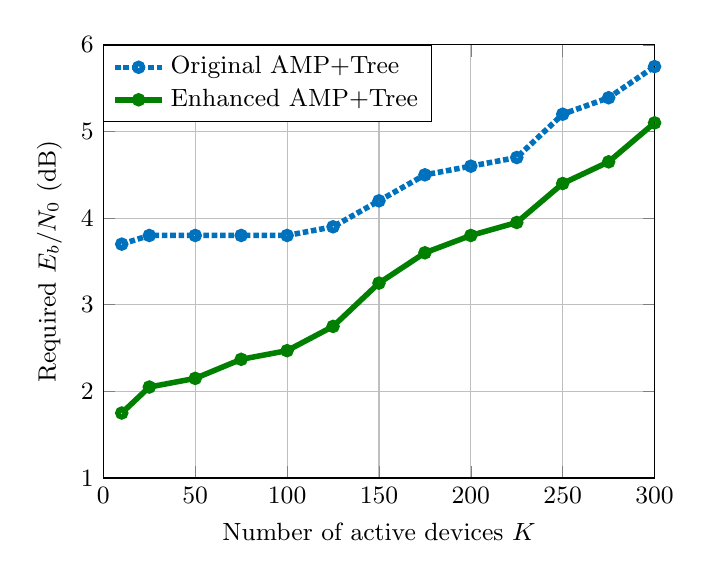
\begin{tikzpicture}
\definecolor{mycolor1}{rgb}{0.63529,0.07843,0.18431}%
\definecolor{mycolor2}{rgb}{0.00000,0.44706,0.74118}%
\definecolor{mycolor3}{rgb}{0.00000,0.49804,0.00000}%
\definecolor{mycolor4}{rgb}{0.87059,0.49020,0.00000}%
\definecolor{mycolor5}{rgb}{0.00000,0.44700,0.74100}%
\definecolor{mycolor6}{rgb}{0.74902,0.00000,0.74902}%

\begin{axis}[%
font=\small,
width=7cm,
height=5.5cm,
scale only axis,
xmin=0,
xmax=300,
xtick = {0,50,100,...,300},
xlabel={Number of active devices $K$},
xmajorgrids,
ymin=1,
ymax=6,
ytick = {1,...,6},
ylabel={Required $E_b/N_0$ (dB)},
ymajorgrids,
legend style={at={(0,1)},anchor=north west, draw=black,fill=white,legend cell align=left}
]



\addplot [color=mycolor2,densely dotted,line width=2.0pt,mark size=1.4pt,mark=o, mark options={solid}]
  table[row sep=crcr]{10 3.7\\
25	3.8\\
50	3.8\\
75	3.8\\
100	3.8\\
125	3.9\\
150	4.2\\
175 4.5\\
200 4.6\\
225 4.7\\
250 5.2\\
275 5.39\\
300 5.75\\
};
\addlegendentry{Original AMP+Tree};

\addplot [color=mycolor3,solid,line width=2.0pt,mark size=1.4pt,mark=o,mark options={solid}]
  table[row sep=crcr]{10 1.75\\
  25  2.05\\
50	2.15\\
75	2.37\\
100	2.47\\
125	2.75\\
150	3.25\\
175 3.6\\
200 3.8\\
225 3.95\\
250 4.4\\
275 4.65\\
300 5.1\\
};
\addlegendentry{Enhanced AMP+Tree};

%\addplot [color=mycolor1,densely dashdotted,line width=2.0pt,mark size=1.4pt,mark=square,mark options={solid}]
%  table[row sep=crcr]{
%  25  2\\
%50	2.1\\
%75	2.2\\
%100	2.41\\
%125	2.57\\
%150	2.81\\
%175	3\\
%200 3.4\\
%225 3.88\\
%250 4.36\\
%275 4.87\\
%300 5.35\\
%};
%\addlegendentry{Sparse IDMA};


\end{axis}


\end{tikzpicture}
}
  \scalebox{0.65}{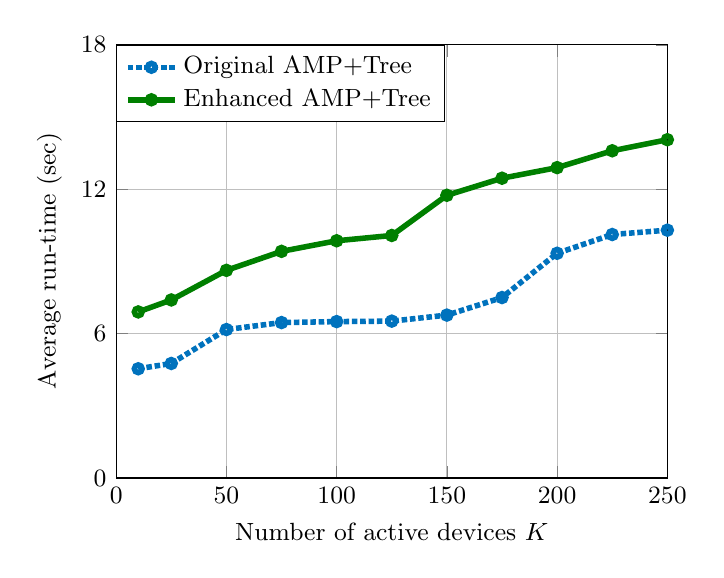
\begin{tikzpicture}
\definecolor{mycolor1}{rgb}{0.63529,0.07843,0.18431}%
\definecolor{mycolor2}{rgb}{0.00000,0.44706,0.74118}%
\definecolor{mycolor3}{rgb}{0.00000,0.49804,0.00000}%
\definecolor{mycolor4}{rgb}{0.87059,0.49020,0.00000}%
\definecolor{mycolor5}{rgb}{0.00000,0.44700,0.74100}%
\definecolor{mycolor6}{rgb}{0.74902,0.00000,0.74902}%

\begin{axis}[%
font=\small,
width=7cm,
height=5.5cm,
scale only axis,
xmin=0,
xmax=250,
xtick = {0,50,100,...,250},
xlabel={Number of active devices $K$},
xmajorgrids,
ymin=0,
ymax=18,
ytick = {0,6,...,18},
ylabel={Average run-time (sec)},
ymajorgrids,
legend style={at={(0,1)},anchor=north west, draw=black,fill=white,legend cell align=left}
]


\addplot [color=mycolor2,densely dotted,line width=2.0pt,mark size=1.4pt,mark=o, mark options={solid}]
  table[row sep=crcr]{10 4.54\\
25	4.76\\
50	6.17\\
75	6.46\\
100	6.5\\
125	6.52\\
150	6.77\\
175 7.5\\
200 9.34\\
225 10.12\\
250 10.3\\
};
\addlegendentry{Original AMP+Tree};

\addplot [color=mycolor3,solid,line width=2.0pt,mark size=1.4pt,mark=o,mark options={solid}]
  table[row sep=crcr]{10 6.903\\
  25  7.4\\
50	8.63\\
75	9.42\\
100	9.86\\
125	10.08\\
150 11.75\\
175 12.46\\
200 12.9\\
225 13.6\\
250 14.06\\
};
\addlegendentry{Enhanced AMP+Tree};
\end{axis}

\end{tikzpicture}
}}
\vspace{5mm}
\begin{itemize}
\item Performance improves significantly with enhanced CCS-AMP decoding
\item Computational complexity is approximately maintained
\item Reparametrization may offer additional gains in performance?
\end{itemize}
\end{frame}

% % % % % % % % % % % % % % % % % % % %

\begin{frame}
\frametitle{CCS and AMP Summary}
% % % % %
\begin{block}{Summary}
\begin{itemize}
\item New connection between CCS and AMP
\item Natural application of BP on factor graph as denoiser
\item Outer code design depends on sparsity
\begin{enumerate}
\item Degree distributions (small graph)
\item Message size (birthday problem)
\item Final step is disambiguation
\end{enumerate}
\item Many theoretical and practical challenges/opportunities exist
\end{itemize}
\end{block}
\begin{center}
\scalebox{0.75}{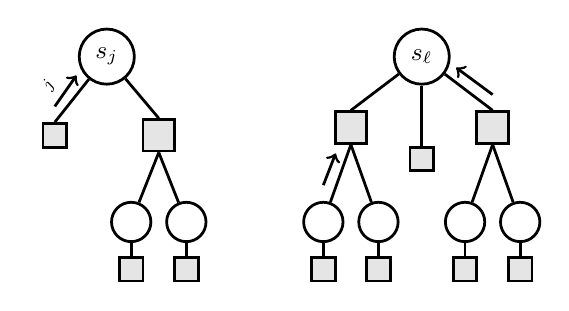
\begin{tikzpicture}
  [
  font=\small, line width=1pt, draw=black,
  check/.style={rectangle, minimum height=4mm, minimum width=4mm, draw=black, fill=gray!20},
  trivialcheck/.style={rectangle, minimum height=3mm, minimum width=3mm, draw=black, fill=gray!20},
  section/.style={circle, minimum size=7mm, draw=black},
  emptysection/.style={circle, minimum size=5mm, draw=black}
  ]

\node[section] (sp) at (0,0) {$s_{j}$};
\node[trivialcheck] (tp) at (-0.66,-1) {};
\node[check] (ap) at (0.66,-1) {};

\node[emptysection] (sp1) at (0.66-0.35,-0.9-1.2) {};
\node[trivialcheck] (tp1) at (0.66-0.35,-1.5-1.2) {}
    edge[-] (sp1);
\node[emptysection] (sp2) at (0.66+0.35,-0.9-1.2) {};
\node[trivialcheck] (tp2) at (0.66+0.35,-1.5-1.2) {}
    edge[-] (sp2);

\draw (sp) -- (tp.north);
\draw (sp) -- (ap.north);
\draw (sp1) -- (ap.south);
\draw (sp2) -- (ap.south);


\node[section] (sl) at (4,0) {$s_{\ell}$};
\node[trivialcheck] (tl) at (4,-1.3) {};
\node[check] (al1) at (4-0.9,-0.9) {};
\node[check] (al2) at (4+0.9,-0.9) {};

\node[emptysection] (sl11) at (3.1-0.35,-0.9-1.2) {};
\node[trivialcheck] (tl11) at (3.1-0.35,-1.5-1.2) {}
    edge[-] (sl11);
\node[emptysection] (sl12) at (3.1+0.35,-0.9-1.2) {};
\node[trivialcheck] (tl12) at (3.1+0.35,-1.5-1.2) {}
    edge[-] (sl12);

\node[emptysection] (sl21) at (4.9-0.35,-0.9-1.2) {};
\node[trivialcheck] (tl21) at (4.9-0.35,-1.5-1.2) {}
    edge[-] (sl21);
\node[emptysection] (sl22) at (4.9+0.35,-0.9-1.2) {};
\node[trivialcheck] (tl22) at (4.9+0.35,-1.5-1.2) {}
    edge[-] (sl22);

\draw (sl) -- (tl.north);
\draw (sl) -- (al1.north);
\draw (sl) -- (al2.north);
\draw (sl11) -- (al1.south);
\draw (sl12) -- (al1.south);
\draw (sl21) -- (al2.south);
\draw (sl22) -- (al2.south);


\draw[shorten <=0.22cm,<-] (sp.south west)++(0,0.2cm) -- node[above,rotate=58,xshift=-0.15cm] {$\lambdav_j$} ([yshift=0.2cm]tp.north);
\draw[shorten <=0.12cm,<-] (al1.south)++(-0.15cm,0) -- node[above,rotate=68,xshift=-0.1cm] {$\lambdav$} ([yshift=0.2cm]sl11.north);
\draw[shorten <=0.22cm,<-] (sl.south east)++(0,0.25cm) -- node[above,rotate=-45,xshift=0.15cm] {${\muv}$} ([yshift=0.2cm]al2.north);

\end{tikzpicture}
}
\end{center}
\centerline{Coding plays increasingly central role in large-scale CS}
\end{frame}

% % % % % % % % % % % % % % % % % % % %

\begin{frame}
\frametitle{Coded Demixing for Single-Class URA}
% % % % %
\begin{columns}
\column{0.52\textwidth}
  \centerline{\begin{tikzpicture}
[font=\footnotesize, draw=black, line width=0.75pt,>=stealth',
sub0/.style={rectangle, draw, inner sep=0pt, minimum width=10mm, minimum height=2.5mm},
parity/.style={rectangle, draw, fill=teal, inner sep=0pt, minimum size=2.5mm}]

\node (cs1) at (0.00,6.125) {Bin~1};
\node (cs2) at (2.00,6.125) {Bin~2};
\node (cs3) at (4.00,6.125) {Bin~3};

\foreach \v in {0.00,2.00,4.00} {
  \draw[->, line width=1pt]  (\v,5.75) -- (\v,5.25);
  \draw[dotted, line width=1pt, draw=gray]  (\v-0.25,5.65) -- (\v,5.25);
  \draw[dotted, line width=1pt, draw=gray]  (\v-0.125,5.7) -- (\v,5.25);
  \draw[dotted, line width=1pt, draw=gray]  (\v+0.125,5.7) -- (\v,5.25);
  \draw[dotted, line width=1pt, draw=gray]  (\v+0.25,5.65) -- (\v,5.25);
}

\foreach \v in {0.00,2.00,4.00} {
  \draw[line width=1pt] (\v-0.375,5) -- (\v-0.5,5) -- (\v-0.5,4.5) -- (\v-0.375,4.5);
  \draw[line width=1pt] (\v+0.375,5) -- (\v+0.5,5) -- (\v+0.5,4.5) -- (\v+0.375,4.5);
  \draw[line width=1pt] (\v+0.575,5) -- (\v+0.575,4) -- (\v+0.7,4) -- (\v+0.7,5) -- (\v+0.575,5);
  \draw[line width=1pt] (\v+0.575,4.25) -- (\v+0.7,4.25);
  \draw[line width=1pt] (\v+0.575,4.5) -- (\v+0.7,4.5);
  \draw[line width=1pt] (\v+0.575,4.75) -- (\v+0.7,4.75);
}

\node at (0.00,4.75) {$\Am_1$};
\node at (2.00,4.75) {$\Am_2$};
\node at (4.00,4.75) {$\Am_{\Theta}$};

\node at (1.1, 4.5) {$+$};
\node at (3.1, 4.5) {$+$};
\end{tikzpicture}
}
  \begin{itemize}
  \item Create multiple bins with (incoherent) matrices
  \item Devices pick a bucket randomly and use CCS-AMP encoding
  \item Perform joint demixing CCS-AMP decoding at access point
  \end{itemize}
\column{0.46\textwidth}
  \centerline{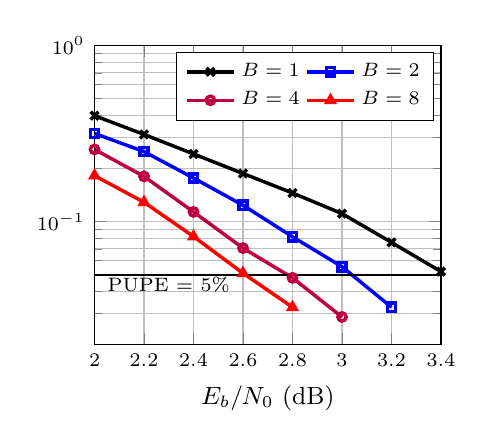
\begin{tikzpicture}

\begin{semilogyaxis}[
font=\small,
width=4.4cm,
height=3.8cm,
scale only axis,
every x tick label/.append style={font=\scriptsize},
xmin=2.0,
xmax=3.4,
xtick={2.0, 2.2, 2.4, 2.6, 2.8, 3.0, 3.2, 3.4},
xlabel={$E_{b}/N_0$ (dB)},
xmajorgrids,
xminorgrids,
every y tick label/.append style={font=\scriptsize},
ymin=0.02,
ymax=1,
ytick={0.01, 0.1, 1.0},
%ylabel={Per-User Probability of Error $P_{\mathrm{e}}$},
ymajorgrids,
yminorgrids,
legend style={anchor=north east,draw=black, fill=white, legend cell align=left,font=\scriptsize, legend columns=2}
]

\addplot [color=black,line width=1.25pt,mark=x]
  table[row sep=crcr]{
  2.0 3.996874999999999734e-01\\
  2.2 3.126562500000000244e-01\\
  2.4 2.423437499999999967e-01\\
  2.6 1.876562499999999967e-01\\
  2.8 1.454687500000000078e-01\\
  3.0 1.110937500000000050e-01\\
  3.2 7.624999999999991507e-02\\
  3.4 5.203124999999998723e-02\\
};
\addlegendentry{$B=1$};

\addplot [color=blue,line width=1.25pt,mark=square,mark size=1.5pt,mark options={solid}]
  table[row sep=crcr]{
  2.0 3.168750000000000733e-01 \\
  2.2 0.24984375\\
  2.4 1.768750000000000322e-01 \\
  2.6 0.12390624999999997 \\
  2.8 8.203124999999994449e-02 \\
  % 3.0 4.749999999999996586e-02 \\
  3.0 0.05546016483516482 \\
  3.2 3.265625000000001860e-02 \\
};
\addlegendentry{$B=2$};

\addplot [color=purple,line width=1.25pt,mark=o,mark size=1.5pt,mark options={solid}]
  table[row sep=crcr]{
  2.0 2.570312500000000999e-01\\
  2.2 0.180665178563 \\
  2.4 1.135937499999999656e-01 \\
  2.6 7.078124999999996225e-02 \\
  2.8 4.796874999999996975e-02 \\
  3.0 2.875000000000002207e-02 \\
};
\addlegendentry{$B=4$};

\addplot [color=red,line width=1.25pt,mark=triangle,mark size=1.5pt,mark options={solid}]
  table[row sep=crcr]{
  2.0 1.824999999999999956e-01 \\
  2.2 1.288194444444443199e-01 \\
  2.4 8.234374999999996558e-02 \\
  2.6 5.093749999999998279e-02 \\
  2.8 3.265625000000001166e-02 \\
};
\addlegendentry{$B=8$};

\draw[black, line width=0.75pt] (axis cs:2,0.05) to (axis cs:3.4,0.05);
\node at (axis cs:2.3,0.044) {\scriptsize PUPE = 5\%};

\end{semilogyaxis}
\end{tikzpicture}
}
\end{columns}
\myfootnote{\tiny
J.~R. Ebert, V.~K. Amalladinne, S. Rini, J.-F. Chamberland, K.~R. Narayanan.
\emph{Stochastic Binning and Coded Demixing for Unsourced Random Access.}
arXiv:2104.05686}
\end{frame}

% % % % % % % % % % % % % % % % % % % %

\begin{frame}
\frametitle{Pertinent References}
\begin{scriptsize}
\begin{itemize}
\item
A.~Fengler, P.~Jung, and G.~Caire.
SPARCs and AMP for Unsourced Random Access.
In \emph{International Symposium on Information Theory (ISIT)}, 2019.

\item
V.~K. Amalladinne, A.~K. Pradhan, C. Rush, J.-F. Chamberland, K.~R. Narayanan.
On approximate message passing for unsourced access with coded compressed sensing.
In \emph{International Symposium on Information Theory (ISIT)}, 2020.

\item
V.~K. Amalladinne, A. Hao, S. Rini, J.-F. Chamberland.
Multi-Class Unsourced Random Access via Coded Demixing.
In \emph{International Symposium on Information Theory (ISIT)}, 2021.

\item
A. Joseph, and A. R. Barron.
Least squares superposition codes of moderate dictionary size are reliable at rates up to capacity
\emph{IEEE Trans.\ on Information Theory}, 2012.

\item
C. Rush, A. Greig, and R. Venkataramanan.
Capacity-achieving sparse superposition codes via approximate message passing decoding.
\emph{IEEE Trans.\ on Information Theory}, 2017.

\item
R. Berthier, A. Montanari, and P.-M. Nguyen.
State Evolution for Approximate Message Passing with Non-Separable Functions.
\emph{Information and Inference: A Journal of the IMA}, 2020.
\end{itemize}
\end{scriptsize}
\end{frame}

% % % % % % % % % % % % % % % % % % % %
